% --------------------------------------------------------------
% This is all preamble stuff that you don't have to worry about.
% Head down to where it says "Start here"
% --------------------------------------------------------------
 
\documentclass[12pt]{article}
 
\usepackage[margin=1in]{geometry} 
\usepackage{amsmath,amsthm,amssymb,scrextend}
\usepackage{fancyhdr}
\usepackage{enumitem}
\usepackage{amsmath}
\usepackage{amssymb}
\usepackage{textcomp}
\usepackage{fancybox}
\usepackage{tikz}
\usepackage{tasks}
\pagestyle{fancy}
\usepackage[makeroom]{cancel}
\usepackage{graphicx}
\usepackage{caption}
\usepackage{mwe}
\usepackage{tikz}
\usetikzlibrary{positioning}

\newcommand{\N}{\mathbb{N}}
\newcommand{\Z}{\mathbb{Z}}
\newcommand{\I}{\mathbb{I}}
\newcommand{\R}{\mathbb{R}}
\newcommand{\Q}{\mathbb{Q}}
\renewcommand{\qed}{\hfill$\blacksquare$}
\let\newproof\proof
\renewenvironment{proof}{\begin{addmargin}[1em]{0em}\begin{newproof}}{\end{newproof}\end{addmargin}\qed}
% \newcommand{\expl}[1]{\text{\hfill[#1]}$}
 
\newenvironment{theorem}[2][Theorem]{\begin{trivlist}
\item[\hskip \labelsep {\bfseries #1}\hskip \labelsep {\bfseries #2.}]}{\end{trivlist}}
\newenvironment{lemma}[2][Lemma]{\begin{trivlist}
\item[\hskip \labelsep {\bfseries #1}\hskip \labelsep {\bfseries #2.}]}{\end{trivlist}}
\newenvironment{problem}[2][Problem]{\begin{trivlist}
\item[\hskip \labelsep {\bfseries #1}\hskip \labelsep {\bfseries #2.}]}{\end{trivlist}}
\newenvironment{exercise}[2][Exercise]{\begin{trivlist}
\item[\hskip \labelsep {\bfseries #1}\hskip \labelsep {\bfseries #2.}]}{\end{trivlist}}
\newenvironment{reflection}[2][Reflection]{\begin{trivlist}
\item[\hskip \labelsep {\bfseries #1}\hskip \labelsep {\bfseries #2.}]}{\end{trivlist}}
\newenvironment{proposition}[2][Proposition]{\begin{trivlist}
\item[\hskip \labelsep {\bfseries #1}\hskip \labelsep {\bfseries #2.}]}{\end{trivlist}}
\newenvironment{corollary}[2][Corollary]{\begin{trivlist}
\item[\hskip \labelsep {\bfseries #1}\hskip \labelsep {\bfseries #2.}]}{\end{trivlist}}
 
\setlength{\parindent}{0pt}
\begin{document}
 \settasks{
	counter-format=(tsk[r]),
	label-width=4ex
}
% --------------------------------------------------------------
%                         Start here
% --------------------------------------------------------------

\lhead{Math 632}
\chead{Homework 8}
\rhead{Meenmo Kang}
\begin{enumerate}
\item Consider an $M/M/\infty$ queue (Durrett Example 4.16) where customers arrive at rate $\lambda$, and the service time for each server is a rate $\mu$ exponential random variable. Let X(t) denote the number of customers in the system at time $t$. Assume that $X(0) = 0$.
\begin{enumerate}[label=(\alph*)]
    \item State the Kolmogorov forward equations for this process.\\
    
    Rates for CTMC
    $$\begin{cases}
    q(n,n+1)=\lambda&\text{for n=0,1,2,...}\\
    q(n,n-1)=n\mu&\text{for n=1,2,3,...}\\
    \end{cases}\quad
    \begin{cases}
    \lambda_0=\lambda\\ \lambda_{n\ge 1} = \lambda + n\mu
    \end{cases}$$
    
    The forward equation
    $$\frac{d}{dt}[p_t(i,j)]=\sum\limits_{k\neq jr} q(i,k)p_t(k,j)-\lambda_i p_t(i,j)$$
    $$\begin{cases}
    j\ge 1: p_t'(i,j) = p_t(i,\;j-1)\lambda+p_t(i,\;j+1)\underbrace{(j+1)\mu}_{n\mu}-(\lambda+j\mu) p_t(i,\;j)\\
    j=0: p_t'(i,0) = p_t(i,1)\mu-\lambda_0 p_t(i,0)
    \end{cases}$$
    
    \vspace{3\baselineskip}
    \item Set $M(t) = E[X(t)]$. Prove that
    $$\frac{dM}{dt} = \lambda - \mu M(t)$$
    {\sl Hint.} Use the equations from (a). Do not hesitate to differentiate series term by term.
    \begin{align}
        \frac{d}{dt}M(t) &= \frac{d}{dt} E[\underbrace{X(t)}_{p_t(0,j)}] = \frac{d}{dt} \sum\limits_{j=0}^\infty jp_t(0,j) = \sum\limits_{j=1}^\infty jp_t'(0,j) \nonumber \\
        &= \sum\limits_{j=1}^\infty j[p_t(0,\;j-1)\lambda+p_t(0,\;j+1)(j+1)\mu - (\lambda+j\mu) p_t(0,\;j)] \nonumber \\
        &=\lambda \underbrace{\sum\limits_{j=1}^\infty(j-1)p_t(0,\;j-1)}_{M(t)}+ \lambda\underbrace{\sum\limits_{j=1}^\infty p_t(0,\;j-1)]}_{1} \nonumber \\
        &+\sum\limits_{j=1}^\infty \mu \underbrace{j(j+1)}_{(j+1)^2-(j+1)}p_t(0,\;j+1) - \lambda \underbrace{\sum\limits_{j=1}^\infty j p_t(0,j)}_{M(t)} - \sum\limits_{j=1}^\infty \mu j^2 p_t(0,j) \nonumber 
    \end{align}
    \begin{align}
    &=\cancel{\lambda\cdot M(t)} + \lambda +\mu \underbrace{\cancel{\sum\limits_{j=1}^\infty (j+1)^2 p_t(0,\;j+1)}}_{p_t(0,1)} -\mu\underbrace{\sum\limits_{j=1}^\infty(j+1)p_t(0,\;j+1)}_{M(t)} \nonumber
    \end{align}
    $$-\cancel{\lambda\cdot M(t)} - \mu\underbrace{\cancel{\sum\limits_{j=1}^\infty j^2p_t(0,\;j)}}_{p_t(0,1)}$$
    \begin{align}
        & = \lambda -\mu M(t) \nonumber a
    \end{align}
    \item Solve the differential equation for M(t). (A reminder about linear ODEs is appended to this HW sheet.)
    \begin{align}
        \frac{dM(t)}{dt} &= \lambda - \mu M(t) \nonumber \\
        e^{\mu t} \frac{dM(t)}{dt} &= e^{\mu t}\lambda - \mu e^{\mu t}M(t) \nonumber \\
        e^{\mu t}\lambda &= \underbrace{e^{\mu t}\frac{dM(t)}{dt} + \mu e^{\mu t}M(t)}_{[e^{\mu t}\cdot M(t)]'}  \nonumber \\
        e^{\mu t}\cdot M(t) &= \int [e^{\mu t}\cdot M(t)]' dt = \int e^{\mu t}\lambda dt = \frac{\lambda}{\mu} e^{\mu t} + C \nonumber \\
        M(t)&= \frac{\lambda}{\mu} + \frac{C}{e^{\mu t}}\quad\Leftrightarrow\quad M(0) = \frac{\lambda}{\mu} + C = 0 \tag*{since X(0)=0} \\
        M(t) &= \frac{\lambda}{\mu}\left(1 - \frac{1}{e^{\mu t}}\right) \nonumber
    \end{align}
    \item Evaluate $\lim\limits_{t\to\infty} M(t)$.The stationary distribution for $X(t)$ is given in Example 4.16 of Durrett's book. Compare the limit you found to the expected value of the stationary distribution.
    $$\lim\limits_{t\to\infty}M(t) = \lim\limits_{t\to\infty} \frac{\lambda}{\mu}\left(1 - \frac{1}{e^{\mu t}}\right) = \frac{\lambda}{\mu}$$
\end{enumerate}
    
\newpage
\item Consider an M/M/2 queue where customers arrive at rate $\lambda$ and the rate for each server
is $\mu$. However, arriving customers who see $N$ customers already in the system leave and
never return. Assume $N > 2$. Let $X(t)$ denote the number of customers in the system at
time $t$. Find the stationary distribution for $X(t)$. (The M/M/s queue appears in Durrett's
examples 4.3 and 4.17.)

$$\begin{cases}
q(n,n+1)=\lambda &\text{for n=0,1,2,...,N-1}\\
q(n,n-1)=\mu &\text{for n=1,2,3,...,N}
\end{cases}$$

Since $\pi\cdot Q = 0$ should be achieved,
$$\begin{bmatrix}
\pi_0&\pi_1&\pi_2&\ldots&\pi_N
\end{bmatrix}
\begin{bmatrix}
-\lambda&\lambda&0&\ldots\\
\mu&-(\mu+\lambda)&\lambda&0&\ldots\\
0&\mu&-(\mu+\lambda)&\lambda&0&\ldots\\
\\
&\ddots&\ddots&\ddots&\ddots&\ddots\\
\\
&&&&\mu&-(\mu+\lambda)&\lambda\\
&&&&0&\mu&-\mu
\end{bmatrix}=
\begin{bmatrix}
0&\ldots&0
\end{bmatrix}$$

\begin{align}
    \lambda\pi_0 = \mu\pi_1 \quad&\Leftrightarrow\quad \pi_1 = \frac{\lambda}{\mu}\pi_0 \nonumber \\
    \lambda\pi_1 = \mu\pi_2 \quad&\Leftrightarrow\quad \pi_2 = \frac{\lambda}{\mu}\pi_1 \nonumber \\
    &\vdots\nonumber \\
    \lambda\pi_{n-1} = \mu\pi_n \quad&\Leftrightarrow\quad \pi_n = \frac{\lambda}{\mu}\pi_{n-1} = \left(\frac{\lambda}{\mu}\right)^n \pi_0 \nonumber \\
    \nonumber \\
    \sum\limits_{j=0}^N\pi_j = 1 \quad&\Leftrightarrow\quad \pi_0\sum\limits_{j=0}^N \left(\frac{\lambda}{\mu}\right)^j =
    \pi_0 \cdot \frac{1-\left(\frac{\lambda}{\mu}\right)^{N+1}}{1-\frac{\lambda}{\mu}} = 1 \nonumber \\
    &\Leftrightarrow \pi_0 =  \frac{1-\frac{\lambda}{\mu}}{1-\left(\frac{\lambda}{\mu}\right)^{N+1}} \nonumber \\
    \nonumber \\
    \pi_j &= \left(\frac{\lambda}{\mu}\right)^j \cdot \frac{1-\frac{\lambda}{\mu}}{1-\left(\frac{\lambda}{\mu}\right)^{N+1}} \nonumber
\end{align}

\newpage
\vspace{2\baselineskip}
For the $M/M/2$ queue, the rates are
$$
            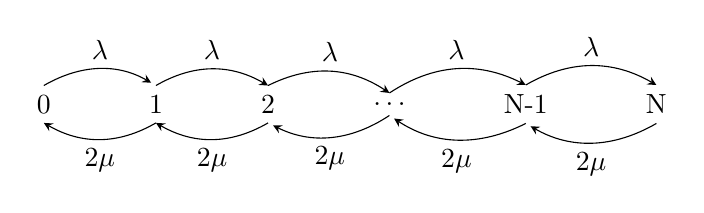
\begin{tikzpicture}
              \node (a) {0};
              \node[right=1cm of a] (b) {1};
              \node[right=1cm of b] (c) {2};
              \node[right=1cm of c] (d) {$\ldots$};
              \node[right=1cm of d] (e) {N-1};
              \node[right=1cm of e] (f) {N};
            
              %a>b
              \draw[-stealth,shorten >= 2pt] (a.north) to[bend left] node[midway,above] {$\lambda$} (b.north);
              \draw[-stealth] (b.north) to[bend left] node[midway,above] {$\lambda$} (c.north);
              \draw[-stealth] (c.north) to[bend left] node[midway,above] {$\lambda$} (d.north);
              \draw[-stealth] (d.north) to[bend left] node[midway,above] {$\lambda$} (e.north);
              \draw[-stealth] (e.north) to[bend left] node[midway,above] {$\lambda$} (f.north);
            
              %b>a
              \draw[-stealth] (b.south) to[bend left] node[midway,below] {2$\mu$} (a.south);
              \draw[-stealth] (c.south) to[bend left] node[midway,below] {2$\mu$} (b.south);
              \draw[-stealth,shorten >= 2pt] (d.south) to[bend left] node[midway,below] {2$\mu$} (c.south);
              \draw[-stealth,shorten >= 2pt] (e.south) to[bend left] node[midway,below] {2$\mu$} (d.south);
              \draw[-stealth,shorten >= 2pt] (f.south) to[bend left] node[midway,below] {2$\mu$} (e.south);
            \end{tikzpicture}
$$

$$\begin{cases}
q(j,\;j+1) = \lambda &\text{for j=0,1,...,N-1}\\
q(j,\;j-1) = 2\mu &\text{for j=2,...,N-1}\\
q(1,0) = \mu
\end{cases}$$

\begin{align}
    \pi(j) &= \frac{q(0,1)q(1,2)\ldots q(j-1,j)}{q(j,j-1)q(j-1,j-2)q(j-2,j-3)\ldots q(1,0)}\cdot \pi(0) \nonumber \\
    &= \frac{\lambda^j}{(2\mu)^{j-1}\mu}\pi(0) = \frac{1}{2^{j-1}} \left(\frac{\lambda}{\mu}\right)^j \pi(0)
    =2\cdot \left(\frac{\lambda}{2\mu}\right)^j \pi(0)    \nonumber\\
    \nonumber \\
    \sum\limits_{j=0}^N \pi(j) &= 1 \quad\Leftrightarrow\quad
    \pi_0 + \sum\limits_{j=0}^N 2\cdot \left(\frac{\lambda}{2\mu}\right)^j \pi(0) =1 \nonumber \\
    &\Leftrightarrow \pi_0\left(1+2\cdot\frac{1-\left(\frac{\lambda}{2\mu}\right)^N}{1-\frac{\lambda}{2\mu}}\cdot \frac{\lambda}{2\mu}     \right)= 1 \nonumber \\
    \pi_0&= \frac{1}{\left(1+2\cdot\frac{1-\left(\frac{\lambda}{2\mu}\right)^N}{1-\frac{\lambda}{2\mu}}\cdot \frac{\lambda}{2\mu}     \right)}\qquad
    \pi_j= 2\left(\frac{\lambda}{2\mu}\right)^j \pi_0 \nonumber 
\end{align}


\newpage
\item 
\begin{enumerate}[label=(\alph*)]
    \item Consider the special case of the previous problem in which $\lambda_1$ = $\lambda_2$ = 1, and $\mu_1$ = $\mu_2$ = 3, and find the stationary probabilities.
    
    $$Q=\begin{pmatrix}
    -2&1&1&0 \\ 
    3&-4&0&1\\
    3&0&-4&1\\ 
    0&3&3&-6
    \end{pmatrix}\qquad
    \pi = \begin{pmatrix}
    \frac{9}{16}&\frac{3}{16}&\frac{3}{16}&\frac{1}{16}
    \end{pmatrix}$$
    \hfill\text{such that $\pi Q = 0$}
    
    \vspace{2\baselineskip}
    \item Suppose they upgrade their telephone system so that a call to one line that is busy is forwarded to the other phone and lost if that phone is busy. Find the new stationary probabilities.
    $$Q=\begin{pmatrix}
    -2&1&1&0 \\ 
    3&-5&0&2\\
    3&0&-5&2\\ 
    0&3&3&-6
    \end{pmatrix}\qquad
    \pi = \begin{pmatrix}
    \frac{9}{17}&\frac{3}{17}&\frac{3}{17}&\frac{2}{17}
    \end{pmatrix}$$
    \hfill\text{such that $\pi Q = 0$}
\end{enumerate}



\newpage
\item A hemoglobin molecule can carry one oxygen or one carbon monoxide molecule. Suppose that the two types of gases arrive at rates 1 and 2 and attach for an exponential amount of time with rates 3 and 4, respectively. Formulate a Markov chain model with state space \{+, 0, \---\} where + denotes an attached oxygen molecule, \---− an attached carbon monoxide molecule, and 0 a free hemoglobin molecule and find the long-run fraction of time the hemoglobin molecule is in each of its three states.

\begin{align}
Q&= \begin{matrix}
&+&0&-\\
+&-3&3&0\\
0&1&-3&2\\
-&0&4&-4
\end{matrix} \nonumber \\
\nonumber \\
\pi &= \begin{bmatrix}
\pi_+&3\pi_+&\frac{3}{2}\pi_+
\end{bmatrix} \tag{such that $\pi Q = 0$} \\
\pi_+ &+ 3\pi_+ + \frac{3}{2}\pi_ = \frac{11}{2} \pi_+ = 1\quad \pi_+ = \frac{2}{11} \nonumber \\
&\Rightarrow \pi = \begin{bmatrix}
\frac{2}{11}&\frac{6}{11}&\frac{3}{11} \nonumber
\end{bmatrix}
\end{align}

\newpage
\item Consider an $M/M/s$ queue with no waiting room. In words, requests for a phone line occur at a rate $\lambda$. If one of the s lines is free, the customer takes it and talks for an exponential amount of time with rate $μ$. If no lines are free, the customer goes away never to come back. Find the stationary distribution. You do not have to evaluate the normalizing constant.

$$
            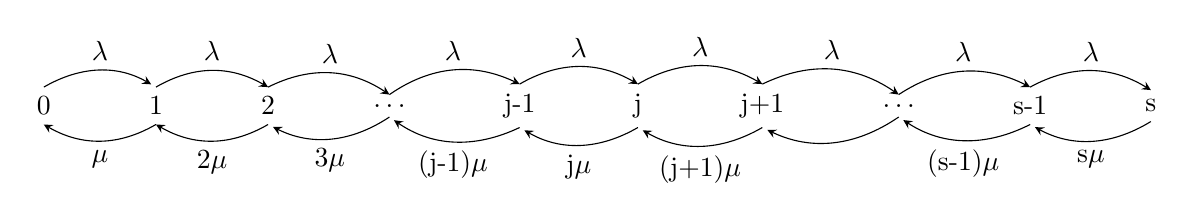
\begin{tikzpicture}
              \node (a) {0};
              \node[right=1cm of a] (b) {1};
              \node[right=1cm of b] (c) {2};
              \node[right=1cm of c] (d) {$\ldots$};
              \node[right=1cm of d] (e) {j-1};
              \node[right=1cm of e] (f) {j};
              \node[right=1cm of f] (g) {j+1};
              \node[right=1cm of g] (h) {$\ldots$};
              \node[right=1cm of h] (i) {s-1};
              \node[right=1cm of i] (j) {s};
            
              %a>b
              \draw[-stealth,shorten >= 2pt] (a.north) to[bend left] node[midway,above] {$\lambda$} (b.north);
              \draw[-stealth] (b.north) to[bend left] node[midway,above] {$\lambda$} (c.north);
              \draw[-stealth] (c.north) to[bend left] node[midway,above] {$\lambda$} (d.north);
              \draw[-stealth] (d.north) to[bend left] node[midway,above] {$\lambda$} (e.north);
              \draw[-stealth] (e.north) to[bend left] node[midway,above] {$\lambda$} (f.north);
              \draw[-stealth] (f.north) to[bend left] node[midway,above] {$\lambda$} (g.north);
              \draw[-stealth] (g.north) to[bend left] node[midway,above] {$\lambda$} (h.north);
              \draw[-stealth] (h.north) to[bend left] node[midway,above] {$\lambda$} (i.north);
              \draw[-stealth] (i.north) to[bend left] node[midway,above] {$\lambda$} (j.north);
            
              %b>a
              \draw[-stealth] (b.south) to[bend left] node[midway,below] {$\mu$} (a.south);
              \draw[-stealth] (c.south) to[bend left] node[midway,below] {2$\mu$} (b.south);
              \draw[-stealth,shorten >= 2pt] (d.south) to[bend left] node[midway,below] {3$\mu$} (c.south);
              \draw[-stealth,shorten >= 2pt] (e.south) to[bend left] node[midway,below] {(j-1)$\mu$} (d.south);
              \draw[-stealth,shorten >= 2pt] (f.south) to[bend left] node[midway,below] {j$\mu$} (e.south);
              \draw[-stealth,shorten >= 2pt] (g.south) to[bend left] node[midway,below] {(j+1)$\mu$} (f.south);
              \draw[-stealth,shorten >= 2pt] (h.south) to[bend left] node[midway,below] {} (g.south);
              \draw[-stealth,shorten >= 2pt] (i.south) to[bend left] node[midway,below] {(s-1)$\mu$} (h.south);
              \draw[-stealth,shorten >= 2pt] (j.south) to[bend left] node[midway,below] {s$\mu$} (i.south);
            \end{tikzpicture}
$$

$$\begin{cases}
q(j,\;j+1)=\lambda &\text{for j=0,1,...,s-1}\\
q(j,\;j-1)=j\mu &\text{for j=1,2,...,s}
\end{cases}$$

Consider the birth and death chain.
\vspace{1\baselineskip}
\begin{align}
  \pi(j) &= \frac{\lambda_{j-1}\ldots\lambda_0}{\mu_j\ldots\mu_1}\pi(0)  \tag{where $q(j,\;j+1)=\lambda_j$ and $q(j,\;j-1)= \mu_j$} \\
  & = \frac{(\lambda_\mu)^j}{j!}\pi(0) \nonumber
\end{align}

\end{enumerate}
\end{document}